\subsection{Sơ đồ và đặc tả use case}

\subsubsection{Sơ đồ use case}

Sơ đồ use case cung cấp cái nhìn tổng quan, cấp cao về ranh giới hệ thống và tất cả các chức năng chính mà hệ thống sẽ thực hiện để đáp ứng nhu cầu của các tác nhân. Hình \ref{fig:use-case-diagram} dưới đây minh họa chi tiết mối quan hệ tương tác này trong ngữ cảnh hệ thống của nhóm.

\begin{figure}[H]
    \centering
    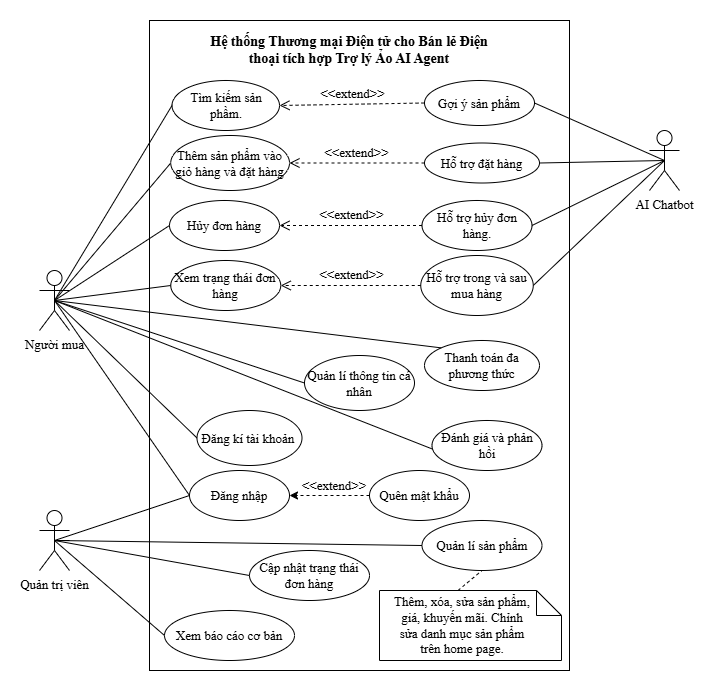
\includegraphics[width=\textwidth]{images/chap3/use_case_diagram/whole_system.png}
    % \vspace{0.5cm}
    \caption{Sơ đồ Use Case tổng thể của hệ thống}
    \label{fig:use-case-diagram}
\end{figure}

\subsubsection{Bảng mô tả chi tiết use case}

{
\fontsize{12pt}{14pt}\selectfont
\renewcommand{\arraystretch}{1.0} 
\setlength{\extrarowheight}{4pt}

\begin{longtable}{|>{\bfseries}p{4cm}|p{11.5cm}|}
\caption{Đặc tả Use Case: Đăng ký tài khoản}
\label{tab:uc-register} \\
\hline
\textbf{Use Case Name} & Đăng ký tài khoản \\
\hline
\textbf{Use Case Overview} & Cho phép khách hàng tạo tài khoản mới. Tài khoản quản trị viên được cấp riêng và không thể tự đăng ký. \\
\hline
\textbf{Actor} & Khách hàng \\
\hline
\textbf{Preconditions} & 1. Hệ thống hoạt động bình thường. \\
& 2. Cơ sở dữ liệu được kết nối với hệ thống. \\
& 3. Kết nối với internet được đảm bảo. \\
& 4. Khách hàng chưa có tài khoản trong hệ thống. \\
\hline
\textbf{Trigger} & Khách hàng nhấn nút “Đăng ký” trên giao diện hệ thống. \\
\hline
\textbf{Steps} & 1. Hệ thống hiển thị biểu mẫu đăng ký. \\
& 2. Khách hàng nhập thông tin bắt buộc (email/số điện thoại, mật khẩu, v.v.). \\
& 3. Hệ thống kiểm tra tính hợp lệ của thông tin. \\
& 4. Hệ thống lưu thông tin khách hàng vào cơ sở dữ liệu. \\
& 5. Hệ thống xác nhận đăng ký thành công. \\
& 6. Khách hàng có thể đăng nhập sau khi xác nhận. \\
\hline
\textbf{Postconditions} & Tài khoản mới được tạo thành công và khách hàng có thể đăng nhập. \\
\hline
\textbf{Alternative Flows} & Không. \\
\hline
\textbf{Exception Flows} & Exception 1: Tại bước 3 \\
& 3a. Nếu email đã tồn tại, hệ thống thông báo (\textit{yêu cầu nhập lại email khác}). \\
& 3b. Nếu mật khẩu không đạt yêu cầu, hệ thống hiển thị thông báo lỗi và yêu cầu đổi mật khẩu khác. \\
& 3c. Nếu các thông tin khác không hợp lệ hoặc chưa điền đủ các trường bắt buộc, hệ thống báo lỗi và yêu cầu nhập chính xác. \\
\hline
\end{longtable}

\begin{longtable}{|>{\bfseries}p{4cm}|p{11.5cm}|}
\caption{Đặc tả Use Case: Đăng nhập}
\label{tab:uc-login} \\
\hline
\textbf{Use Case Name} & Đăng nhập \\
\hline
\textbf{Use Case Overview} & Cho phép người dùng đăng nhập vào hệ thống bằng tài khoản đã đăng ký. \\
\hline
\textbf{Actor} & Khách hàng, Quản trị viên \\
\hline
\textbf{Preconditions} & 1. Hệ thống hoạt động bình thường. \\
& 2. Cơ sở dữ liệu được kết nối với hệ thống. \\
& 3. Kết nối với internet được đảm bảo. \\
& 4. Người dùng đã có tài khoản trong hệ thống.\\
\hline
\textbf{Trigger} & Người dùng nhấn nút “Đăng nhập” trên giao diện hệ thống. \\
\hline
\textbf{Steps} & 1. Hệ thống hiển thị màn hình đăng nhập. \\
& 2. Người dùng nhập thông tin đăng nhập. \\
& 3. Hệ thống xác thực thông tin đăng nhập. \\
& 4. Người dùng được chuyển đến trang chủ nếu đăng nhập thành công. \\
\hline
\textbf{Postconditions} & Người dùng đã đăng nhập thành công vào hệ thống. \\
\hline
\textbf{Alternative Flows} & Alternative 1: Tại bước 2 \\
& 2a. Đối với người dùng là khách hàng, nếu quên mật khẩu, khách hàng nhấn chọn nút “Quên mật khẩu” để chuyển đến trang cấp lại mật khẩu. \\
& 2b. Đối với người dùng là khách hàng, nếu chọn phương thức đăng nhập bằng Google, hệ thống sẽ chuyển đến trang xác thực của Google\\
\hline
\textbf{Exception Flows} & Exception 1: Tại bước 3 \\
& 3a. Thông tin đăng nhập không hợp lệ (sai tên tài khoản hoặc mật khẩu), hệ thống hiển thị thông báo lỗi và yêu cầu người dùng thử lại. \\
\hline
\end{longtable}

\begin{longtable}{|>{\bfseries}p{4cm}|p{11.5cm}|}
\caption{Đặc tả Use Case: Quên mật khẩu}
\label{tab:uc-forgot-password} \\
\hline
\textbf{Use Case Name} & Quên mật khẩu \\
\hline
\textbf{Use Case Overview} & Cho phép khách hàng lấy lại mật khẩu đã quên. \\
\hline
\textbf{Actor} & Khách hàng\\
\hline
\textbf{Preconditions} & 1. Hệ thống hoạt động bình thường. \\
& 2. Cơ sở dữ liệu được kết nối với hệ thống. \\
& 3. Kết nối với internet được đảm bảo. \\
& 4. Người dùng đã có tài khoản trong hệ thống. \\
\hline
\textbf{Trigger} & Khách hàng nhấn nút “Quên mật khẩu”. \\
\hline
\textbf{Steps} & 1. Hệ thống hiển thị màn hình quên mật khẩu. \\
& 2. Khách hàng nhập thông tin email hoặc số điện thoại đã đăng ký tài khoản. \\
& 3. Hệ thống xác thực thông tin. \\
& 4. Hệ thống gửi đường dẫn đến trang đổi mật khẩu đến email hoặc sms của khách hàng. \\
& 5. Khách hàng nhập mật khẩu mới. \\
& 6. Hệ thống kiểm tra và cập nhật mật khẩu mới. \\
\hline
\textbf{Postconditions} & Khách hàng thiết lập mật khẩu mới thành công. \\
\hline
\textbf{Alternative Flows} & Không \\
\hline
\textbf{Exception Flows} & Exception 1: Tại bước 3 \\
& 3a. Thông tin email và số điện thoại không đúng. \\
& Exception 2: Tại bước 6 \\
& 6a. Mật khẩu mới không hợp lệ. \\
\hline
\end{longtable}

\begin{longtable}{|>{\bfseries}p{4cm}|p{11.5cm}|}
\caption{Đặc tả Use Case: Quản lý thông tin cá nhân}
\label{tab:uc-profile-management} \\
\hline
\textbf{Use Case Name} & Quản lý thông tin cá nhân \\
\hline
\textbf{Use Case Overview} & Khách hàng xem và cập nhật thông tin cá nhân. \\
\hline
\textbf{Actor} & Khách hàng. \\
\hline
\textbf{Preconditions} & 1. Hệ thống hoạt động bình thường. \\
& 2. Cơ sở dữ liệu được kết nối với hệ thống. \\
& 3. Kết nối với internet được đảm bảo. \\
& 4. Khách hàng đã đăng nhập thành công. \\
\hline
\textbf{Trigger} & Khách hàng truy cập mục “Thông tin cá nhân”. \\
\hline
\textbf{Steps} & 1. Hệ thống hiển thị thông tin cá nhân hiện tại. \\
& 2. Khách hàng chọn chỉnh sửa thông tin. \\
& 3. Khách hàng nhập thông tin mới. \\
& 4. Hệ thống lưu thay đổi và cập nhật hồ sơ. \\
\hline
\textbf{Postconditions} & Thông tin cá nhân mới được cập nhật thành công. \\
\hline
\textbf{Alternative Flows} & Alternative 1: Tại bước 2 \\
& 2a. Nếu khách hàng chỉ xem lại thông tin cá nhân mà không cần chỉnh sửa thì không chọn nút chỉnh sửa thông tin cá nhân. \\
\hline
\textbf{Exception Flows} & Exception 1: Tại bước 3 \\
& 3a. Thông tin cập nhật không hợp lệ, hệ thống báo lỗi. \\
\hline
\end{longtable}

\begin{longtable}{|>{\bfseries}p{4cm}|p{11.5cm}|}
\caption{Đặc tả Use Case: Tìm kiếm sản phẩm}
\label{tab:uc-search-product} \\
\hline
\textbf{Use Case Name} & Tìm kiếm sản phẩm \\
\hline
\textbf{Use Case Overview} & Cho phép khách hàng tìm kiếm sản phẩm theo từ khóa hoặc tiêu chí. \\
\hline
\textbf{Actor} & Khách hàng. \\
\hline
\textbf{Preconditions} & 1. Hệ thống hoạt động bình thường. \\
& 2. Cơ sở dữ liệu được kết nối với hệ thống. \\
& 3. Kết nối với internet được đảm bảo. \\
\hline
\textbf{Trigger} & Khách hàng nhập từ khóa vào thanh tìm kiếm hoặc chọn tiêu chí tìm kiếm. \\
\hline
\textbf{Steps} & 1. Khách hàng nhập từ khóa hoặc chọn bộ lọc sản phẩm. \\
& 2. Hệ thống truy vấn cơ sở dữ liệu để tìm sản phẩm phù hợp. \\
& 3. Hệ thống hiển thị danh sách sản phẩm. \\
\hline
\textbf{Postconditions} & Danh sách sản phẩm hiển thị phù hợp với tiêu chí tìm kiếm của khách hàng. \\
\hline
\textbf{Alternative Flows} & Không. \\
\hline
\textbf{Exception Flows} & Exception 1: Tại bước 2 \\
& 2a. Nếu có lỗi kết nối cơ sở dữ liệu, hệ thống báo lỗi và yêu cầu thử lại. \\
& Exception 2: Tại bước 3 \\
& 3a. Nếu có sản phẩm phù hợp, hệ thống hiển thị thông báo. \\
\hline
\end{longtable}

\begin{longtable}{|>{\bfseries}p{4cm}|p{11.5cm}|}
\caption{Đặc tả Use Case: Gợi ý sản phẩm}
\label{tab:uc-product-suggestion} \\
\hline
\textbf{Use Case Name} & Gợi ý sản phẩm \\
\hline
\textbf{Use Case Overview} & Hệ thống AI ChatBot phân tích hành vi, lịch sử mua sắm và từ khóa tìm kiếm để đưa ra gợi ý sản phẩm cá nhân hóa. Đây là use case mở rộng từ “Tìm kiếm sản phẩm”. \\
\hline
\textbf{Actor} & AI ChatBot. \\
\hline
\textbf{Preconditions} & 1. Hệ thống hoạt động bình thường. \\
& 2. Cơ sở dữ liệu được kết nối với hệ thống. \\
& 3. Kết nối với internet được đảm bảo. \\
& 4. Use case “Tìm kiếm và so sánh sản phẩm” đã được khởi động. \\
& 5. Dữ liệu hành vi và lịch sử khách hàng được lưu trữ. \\
& 6. AI ChatBot hoạt động và có quyền truy cập dữ liệu sản phẩm. \\
\hline
\textbf{Trigger} & Khách hàng tương tác với ChatBot. \\
\hline
\textbf{Steps} & 1. AI ChatBot phân tích từ khóa, lịch sử mua sắm, và hành vi duyệt web. \\
& 2. Hệ thống hiển thị câu trả lời chứa gợi ý sản phẩm trong hộp thoại chat. \\
\hline
\textbf{Postconditions} & Gợi ý sản phẩm cá nhân hóa được hiển thị cho khách hàng. \\
\hline
\textbf{Alternative Flows} & Không. \\
\hline
\textbf{Exception Flows} & Exception 1: Tại bước 2 \\
& 2a. Nếu có lỗi kết nối cơ sở dữ liệu, hệ thống báo lỗi và yêu cầu thử lại. \\
& Exception 2: Tại bước 3 \\
& 3a. Nếu không có sản phẩm phù hợp, hệ thống hiển thị thông báo. \\
\hline
\end{longtable}

\begin{longtable}{|>{\bfseries}p{4cm}|p{11.5cm}|}
\caption{Đặc tả Use Case: Thêm sản phẩm vào giỏ hàng và đặt hàng}
\label{tab:uc-add-to-cart-checkout} \\
\hline
\textbf{Use Case Name} & Thêm sản phẩm vào giỏ hàng và đặt hàng \\
\hline
\textbf{Use Case Overview} & Cho phép khách hàng lựa chọn sản phẩm, thêm vào giỏ hàng và thực hiện quy trình đặt hàng với nhiều phương thức thanh toán khác nhau. \\
\hline
\textbf{Actor} & Khách hàng \\
\hline
\textbf{Preconditions} & 1. Hệ thống hoạt động bình thường. \\
& 2. Cơ sở dữ liệu được kết nối với hệ thống. \\
& 3. Kết nối với internet được đảm bảo. \\
& 4. Sản phẩm còn hàng. \\
\hline
\textbf{Trigger} & Khách hàng chọn sản phẩm và nhấn nút “Thêm vào giỏ hàng” hoặc “Đặt hàng”. \\
\hline
\textbf{Steps} & 1. Khách hàng chọn sản phẩm cần mua. \\
& 2. Hệ thống hiển thị chi tiết sản phẩm và nút “Thêm vào giỏ hàng”. \\
& 3. Khách hàng thêm sản phẩm vào giỏ. \\
& 4. Hệ thống cập nhật giỏ hàng và hiển thị tổng số lượng, giá tiền. \\
& 5. Khách hàng chọn “Đặt hàng”. \\
& 6. Hệ thống yêu cầu khách hàng xác nhận địa chỉ giao hàng, phương thức thanh toán. \\
& 7. Hệ thống kiểm tra tính hợp lệ của thông tin và số lượng tồn kho. \\
& 8. Hệ thống tạo đơn hàng và gửi xác nhận cho khách hàng. \\
\hline
\textbf{Postconditions} & Đơn hàng được tạo thành công và lưu trong hệ thống, khách hàng nhận thông báo xác nhận. \\
\hline
\textbf{Alternative Flows} & Alternative 1: Tại bước 4 \\
& 4a. Khách hàng không đặt hàng ngay mà chỉ thêm sản phẩm vào giỏ hàng. \\
\hline
\textbf{Exception Flows} & Exception 1: Tại bước 6 \\
& 6a. Nếu phương thức thanh toán hiện tại không hỗ trợ, hệ thống báo lỗi và yêu cầu khách hàng chọn phương thức thanh toán khác. \\
\hline
\end{longtable}

\begin{longtable}{|>{\bfseries}p{4cm}|p{11.5cm}|}
\caption{Đặc tả Use Case: Hỗ trợ đặt hàng}
\label{tab:uc-chatbot-order-support} \\
\hline
\textbf{Use Case Name} & Hỗ trợ đặt hàng \\
\hline
\textbf{Use Case Overview} & AI ChatBot dựa vào tin nhắn của khách hàng từ đó xác định nhu cầu của khách hàng và gửi đề xuất cho đặt hàng cho khách hàng. \\
\hline
\textbf{Actor} & AI ChatBot. \\
\hline
\textbf{Preconditions} & 1. Hệ thống hoạt động bình thường. \\
& 2. Cơ sở dữ liệu được kết nối với hệ thống. \\
& 3. Kết nối với internet được đảm bảo. \\
& 4. Use case “Thêm sản phẩm vào giỏ hàng và đặt hàng” đã được khởi động. \\
& 5. AI ChatBot hoạt động bình thường và được tích hợp vào hệ thống. \\
& 6. Dữ liệu sản phẩm và lịch sử khách hàng khả dụng để phân tích. \\
\hline
\textbf{Trigger} & Khách hàng trò chuyện với AI ChatBot và có yêu cầu đặt hàng. \\
\hline
\textbf{Steps} & 1. Khách hàng gửi các tin nhắn về nhu cầu đặt hàng để AI có đủ thông tin về đơn hàng. \\
& 2. AI ChatBot đưa ra thông tin về đơn hàng và hiển thị cửa sổ xác nhận. \\
& 3. Khách hàng có thể chọn “đồng ý” để tiến hành đặt hàng hoặc “không đồng ý”. \\
& 4. Hệ thống tiếp tục quy trình đặt hàng. \\
\hline
\textbf{Postconditions} & Nếu khách hàng đồng ý, đơn hàng được xác nhận và hệ thống chuyển sang quy trình đặt hàng chính thức. Ngược lại, không có đơn hàng nào được tạo. Đồng thời hệ thống lưu lại lịch sử tương tác để cải thiện gợi ý trong tương lai. \\
\hline
\textbf{Alternative Flows} & Không. \\
\hline
\textbf{Exception Flows} & Exception 1: Tại bước 2 \\
& 2a. Nếu xảy ra các lỗi về kết nối, truy xuất dữ liệu, hệ thống báo lỗi. \\
\hline
\end{longtable}

\vspace{2em}

\begin{longtable}{|>{\bfseries}p{4cm}|p{11.5cm}|}
\caption{Đặc tả Use Case: Thanh toán đa phương thức}
\label{tab:uc-multipayment} \\
\hline
\textbf{Use Case Name} & Thanh toán đa phương thức \\
\hline
\textbf{Use Case Overview} & Cho phép khách hàng thanh toán đơn hàng bằng nhiều phương thức khác nhau như: tiền mặt khi nhận hàng (COD), thẻ ngân hàng, ví điện tử, hoặc các cổng thanh toán trực tuyến. \\
\hline
\textbf{Actor} & Khách hàng. \\
\hline
\textbf{Preconditions} & 1. Hệ thống hoạt động bình thường. \\
& 2. Cơ sở dữ liệu được kết nối với hệ thống. \\
& 3. Kết nối với Internet được đảm bảo. \\
& 4. Đơn hàng đã được tạo thành công. \\
& 5. Hệ thống kết nối với các cổng thanh toán bên thứ ba (nếu có). \\
\hline
\textbf{Trigger} & Khách hàng chọn “Thanh toán” sau khi xác nhận đơn hàng đối với các phương thức trả trước. \\
\hline
\textbf{Steps} & 1. Tùy vào phương thức thanh toán mà khách hàng chọn, thông tin thanh toán sẽ hiển thị ra màn hình. \\
& 2. Khách hàng thực hiện thanh toán. \\
& 3. Hệ thống hiển thị trạng thái thanh toán và cập nhật trạng thái đơn hàng. \\
\hline
\textbf{Postconditions} & Thanh toán được xử lý thành công và lưu vào hệ thống. \\
\hline
\textbf{Alternative Flows} & Alternative 1: Tại bước 2 \\
& 2a. Nếu phương thức thanh toán là “Thanh toán khi nhận hàng”, khách hàng bỏ qua bước 2, đơn hàng tự động cập nhật trạng thái. \\
\hline
\textbf{Exception Flows} & Exception 1: Tại bước 2 \\
& 2a. Thanh toán thất bại (sai OTP, số dư không đủ), hệ thống báo lỗi và yêu cầu thử lại hoặc chọn phương thức khác. \\
& 2b. Lỗi kết nối với cổng thanh toán, hệ thống hiển thị thông báo và giữ đơn hàng ở trạng thái “Chờ thanh toán”. \\
\hline
\end{longtable}

\begin{longtable}{|>{\bfseries}p{4cm}|p{11.5cm}|}
\caption{Đặc tả Use Case: Hủy đơn hàng}
\label{tab:uc-cancel-order} \\
\hline
\textbf{Use Case Name} & Hủy đơn hàng \\
\hline
\textbf{Use Case Overview} & Cho phép khách hàng hủy đơn hàng đã đặt trong một số điều kiện nhất định \\
\hline
\textbf{Actor} & Khách hàng. \\
\hline
\textbf{Preconditions} & 1. Hệ thống hoạt động bình thường. \\
& 2. Cơ sở dữ liệu được kết nối với hệ thống. \\
& 3. Kết nối với Internet được đảm bảo. \\
& 4. Đơn hàng ở trạng thái được cho phép hủy. \\
\hline
\textbf{Trigger} & Khách hàng chọn hủy đơn hàng. \\
\hline
\textbf{Steps} & 1. Khách hàng mở danh sách đơn hàng và chọn đơn hàng muốn hủy. \\
& 2. Hệ thống hiển thị chi tiết đơn hàng. \\
& 3. Khách hàng nhấn nút “Hủy đơn hàng”. \\
& 4. Hệ thống yêu cầu khách hàng xác nhận lý do hủy. \\
& 5. Hệ thống kiểm tra điều kiện hủy. \\
& 6. Hệ thống thay đổi trạng thái đơn hàng thành “Đã hủy” và gửi thông báo xác nhận cho khách hàng. \\
\hline
\textbf{Postconditions} & Đơn hàng được hủy thành công và không tiếp tục xử lý. \\
\hline
\textbf{Alternative Flows} & Alternative 1: Tại bước 4 \\
& 4a. Khách hàng từ chối hủy sau bước 4, hệ thống giữ nguyên trạng thái đơn hàng. \\
\hline
\textbf{Exception Flows} & Exception 1: Tại bước 5 \\
& 5a. Đơn hàng không còn ở trạng thái cho phép hủy, hệ thống thông báo đơn hàng không thể hủy cho khách hàng. \\
& 5b. Lỗi kết nối cơ sở dữ liệu, hệ thống hiển thị thông báo lỗi và không thay đổi trạng thái đơn hàng. \\
\hline
\end{longtable}

\begin{longtable}{|>{\bfseries}p{4cm}|p{11.5cm}|}
\caption{Đặc tả Use Case: Hỗ trợ hủy đơn hàng}
\label{tab:uc-chatbot-cancel-support} \\
\hline
\textbf{Use Case Name} & Hỗ trợ hủy đơn hàng \\
\hline
\textbf{Use Case Overview} & AI ChatBot hỗ trợ giúp khách hàng hủy đơn hàng nếu họ gặp khó khăn trong quá trình hủy đơn hàng. Đây là use case mở rộng từ “Hủy đơn hàng”. \\
\hline
\textbf{Actor} & AI ChatBot \\
\hline
\textbf{Preconditions} & 1. Hệ thống hoạt động bình thường. \\
& 2. Cơ sở dữ liệu được kết nối với hệ thống. \\
& 3. Kết nối với Internet được đảm bảo. \\
& 4. Use case “Hủy đơn hàng” đã được khởi động. \\
& 5. AI ChatBot khả dụng. \\
& 6. Đơn hàng ở trạng thái có thể hủy. \\
\hline
\textbf{Trigger} & Khách hàng yêu cầu trợ giúp khi muốn hủy đơn hàng. \\
\hline
\textbf{Steps} & 1. Khách hàng gửi yêu cầu hủy đơn hàng cho AI ChatBot. \\
& 2. AI ChatBot hiển thị thông tin đơn hàng và hỏi xác nhận từ khách hàng. \\
& 3. Khách hàng xác nhận hủy. \\
& 4. Hệ thống kiểm tra điều kiện hủy. \\
& 5. Nếu hợp lệ, hệ thống thay đổi trạng thái đơn hàng thành “Đã hủy”. \\
& 6. AI ChatBot thông báo kết quả hủy đơn hàng cho khách hàng. \\
\hline
\textbf{Postconditions} & Đơn hàng được hủy thành công thông qua thao tác của AI ChatBot. \\
\hline
\textbf{Alternative Flows} & Alternative 1: Tại bước 3 \\
& 3a. Khách hàng từ chối xác nhận lại bước 3, hệ thống giữ nguyên trạng thái đơn hàng. \\
\hline
\textbf{Exception Flows} & Exception 1: Tại bước 5 \\
& 5a. Đơn hàng không còn ở trạng thái cho phép hủy, hệ thống thông báo đơn hàng không thể hủy cho khách hàng. \\
& 5b. Lỗi kết nối cơ sở dữ liệu, hệ thống hiển thị thông báo lỗi và không thay đổi trạng thái đơn hàng. \\
\hline
\end{longtable}

\begin{longtable}{|>{\bfseries}p{4cm}|p{11.5cm}|}
\caption{Đặc tả Use Case: Xem trạng thái đơn hàng}
\label{tab:uc-view-order-status} \\
\hline
\textbf{Use Case Name} & Xem trạng thái đơn hàng \\
\hline
\textbf{Use Case Overview} & Cho phép khách hàng theo dõi tiến trình đơn hàng sau khi đặt (chờ xác nhận, đang giao, đã giao thành công hoặc hủy). \\
\hline
\textbf{Actor} & Khách hàng \\
\hline
\textbf{Preconditions} & 1. Hệ thống hoạt động bình thường. \\
& 2. Cơ sở dữ liệu được kết nối với hệ thống. \\
& 3. Kết nối với Internet được đảm bảo. \\
& 4. Khách hàng đã đăng nhập vào hệ thống. \\
\hline
\textbf{Trigger} & Khách hàng chọn chức năng “Xem đơn hàng” trên giao diện. \\
\hline
\textbf{Steps} & 1. Khách hàng truy cập mục đơn hàng có trạng thái cần xem. \\
& 2. Hệ thống hiển thị danh sách đơn hàng gần nhất phù hợp. \\
& 3. Khách hàng chọn một đơn hàng cụ thể. \\
& 4. Hệ thống hiển thị chi tiết trạng thái đơn hàng. \\
\hline
\textbf{Postconditions} & Khách hàng biết được trạng thái và tiến trình xử lý đơn hàng. \\
\hline
\textbf{Alternative Flows} & Không. \\
\hline
\textbf{Exception Flows} & Exception 1: Tại bước 2 \\
& 2a. Nếu không có đơn hàng nào phù hợp, hệ thống hiển thị danh sách rỗng và thông báo. \\
\hline
\end{longtable}

\begin{longtable}{|>{\bfseries}p{4cm}|p{11.5cm}|}
\caption{Đặc tả Use Case: Hỗ trợ trong và sau mua hàng}
\label{tab:uc-post-purchase-support} \\
\hline
\textbf{Use Case Name} & Hỗ trợ trong và sau mua hàng \\
\hline
\textbf{Use Case Overview} & AI ChatBot hoặc nhân viên hỗ trợ cung cấp thông tin, tư vấn và giải đáp thắc mắc liên quan đến đơn hàng trong quá trình xử lý hoặc sau khi hoàn tất. Đây là use case mở rộng từ “Xem trạng thái đơn hàng”. \\
\hline
\textbf{Actor} & AI ChatBot. \\
\hline
\textbf{Preconditions} & 1. Hệ thống hoạt động bình thường. \\
& 2. Cơ sở dữ liệu được kết nối với hệ thống. \\
& 3. Kết nối với Internet được đảm bảo. \\
& 4. Use case “Xem trạng thái đơn hàng” đã được khởi động. \\
& 5. AI ChatBot khả dụng. \\
& 6. Dữ liệu đơn hàng và lịch sử tương tác được lưu trữ trong hệ thống. \\
\hline
\textbf{Trigger} & Khách hàng yêu cầu Chatbot hỗ trợ khi đang xem chi tiết đơn hàng. \\
\hline
\textbf{Steps} & 1. Khách hàng chọn nút “Trợ giúp” hoặc nhắn tin trong giao diện ChatBot. \\
& 2. AI ChatBot phân tích yêu cầu và đưa ra phản hồi tự động. \\
\hline
\textbf{Postconditions} & Khách hàng nhận được thông tin hỗ trợ hoặc giải pháp cho vấn đề liên quan đến đơn hàng. \\
\hline
\textbf{Alternative Flows} & Alternative 1: Tại bước 2 \\
& 4a. Khách hàng chỉ cần tham khảo FAQ, AI ChatBot cung cấp liên kết đến trang hướng dẫn. \\
\hline
\textbf{Exception Flows} & Exception 1: Tại bước 2 \\
& 2a. ChatBot không sẵn có và có lỗi trong kết nối, hệ thống báo lỗi và cho phép khách hàng gửi yêu cầu hỗ trợ qua email. \\
\hline
\end{longtable}

\begin{longtable}{|>{\bfseries}p{4cm}|p{11.5cm}|}
\caption{Đặc tả Use Case: Đánh giá và phản hồi của khách hàng}
\label{tab:uc-customer-review} \\
\hline
\textbf{Use Case Name} & Đánh giá và phản hồi của khách hàng \\
\hline
\textbf{Use Case Overview} & Khách hàng có thể gửi đánh giá (sao, nhận xét) về sản phẩm hoặc dịch vụ sau khi nhận hàng để cải thiện chất lượng hệ thống. \\
\hline
\textbf{Actor} & Khách hàng. \\
\hline
\textbf{Preconditions} & 1. Hệ thống hoạt động bình thường. \\
& 2. Cơ sở dữ liệu được kết nối với hệ thống. \\
& 3. Kết nối với Internet được đảm bảo. \\
& 4. Khách hàng đã đăng nhập. \\
\hline
\textbf{Trigger} & Khách hàng chọn chức năng “Đánh giá/Phản hồi” trong mục đơn hàng đã hoàn tất. \\
\hline
\textbf{Steps} & 1. Hệ thống hiển thị biểu mẫu đánh giá sản phẩm. \\
& 2. Khách hàng nhập số sao, nhận xét hoặc góp ý. \\
& 3. Hệ thống lưu phản hồi vào cơ sở dữ liệu và xác nhận đánh giá thành công. \\
\hline
\textbf{Postconditions} & Đánh giá và phản hồi được lưu trong hệ thống, có thể hiển thị công khai hoặc nội bộ. \\
\hline
\textbf{Alternative Flows} & Alternative 1: Tại bước 1 \\
& 4a. Khách hàng bỏ qua bước đánh giá, đơn hàng vẫn hoàn tất nhưng không có phản hồi. \\
\hline
\textbf{Exception Flows} & Không. \\
\hline
\end{longtable}

\begin{longtable}{|>{\bfseries}p{4cm}|p{11.5cm}|}
\caption{Đặc tả Use Case: Quản lý sản phẩm}
\label{tab:uc-admin-product-management} \\
\hline
\textbf{Use Case Name} & Quản lý sản phẩm \\
\hline
\textbf{Use Case Overview} & Cho phép quản trị viên thêm mới, chỉnh sửa thông tin, hoặc xóa sản phẩm trong hệ thống. \\
\hline
\textbf{Actor} & Quản trị viên. \\
\hline
\textbf{Preconditions} & 1. Hệ thống hoạt động bình thường. \\
& 2. Cơ sở dữ liệu được kết nối với hệ thống. \\
& 3. Kết nối với Internet được đảm bảo. \\
& 4. Quản trị viên đã đăng nhập vào hệ thống. \\
\hline
\textbf{Trigger} & Quản trị viên chọn chức năng “Quản lý sản phẩm” trong giao diện quản trị. \\
\hline
\textbf{Steps} & 1. Quản trị viên chọn thêm mới, chỉnh sửa hoặc xóa sản phẩm. \\
& 2. Hệ thống hiển thị biểu mẫu tương ứng. \\
& 3. Quản trị viên nhập hoặc cập nhật thông tin sản phẩm. \\
& 4. Hệ thống kiểm tra tính hợp lệ dữ liệu. \\
& 5. Hệ thống lưu thông tin sản phẩm vào cơ sở dữ liệu. \\
& 6. Hệ thống xác nhận thao tác thành công. \\
\hline
\textbf{Postconditions} & Danh mục sản phẩm được cập nhật trong hệ thống. \\
\hline
\textbf{Alternative Flows} & Alternative 1: Tại bước 3 \\
& 3a. Quản trị viên hủy thao tác trước khi lưu, không có thay đổi nào được thực hiện. \\
\hline
\textbf{Exception Flows} & Exception 1: Tại bước 4 \\
& 4a. Nếu dữ liệu được nhập không hợp lệ, hệ thống báo lỗi và yêu cầu quản trị viên nhập lại. \\
\hline
\end{longtable}

\begin{longtable}{|>{\bfseries}p{4cm}|p{11.5cm}|}
\caption{Đặc tả Use Case: Cập nhật trạng thái đơn hàng}
\label{tab:uc-admin-update-order-status} \\
\hline
\textbf{Use Case Name} & Cập nhật trạng thái đơn hàng \\
\hline
\textbf{Use Case Overview} & Cho phép quản trị viên hoặc nhân viên vận hành thay đổi trạng thái đơn hàng (xác nhận, đang giao, đã giao, hủy). \\
\hline
\textbf{Actor} & Quản trị viên. \\
\hline
\textbf{Preconditions} & 1. Hệ thống hoạt động bình thường. \\
& 2. Cơ sở dữ liệu được kết nối với hệ thống. \\
& 3. Kết nối với Internet được đảm bảo. \\
& 4. Quản trị viên đã đăng nhập vào hệ thống. \\
\hline
\textbf{Trigger} & Quản trị viên chọn đơn hàng cụ thể từ danh sách để cập nhật trạng thái. \\
\hline
\textbf{Steps} & 1. Quản trị viên truy cập danh sách đơn hàng. \\
& 2. Hệ thống hiển thị chi tiết đơn hàng. \\
& 3. Quản trị viên chọn trạng thái mới. \\
& 4. Hệ thống cập nhật cơ sở dữ liệu. \\
& 5. Hệ thống thông báo cho khách hàng về trạng thái mới. \\
\hline
\textbf{Postconditions} & Đơn hàng được cập nhật trạng thái thành công trong hệ thống. \\
\hline
\textbf{Alternative Flows} & Không. \\
\hline
\textbf{Exception Flows} & Exception 1: Tại bước 3 \\
& 3a. Nếu đơn hàng bị hủy ngay khi quản trị viên đang cập nhật, hệ thống hiển thị lỗi. \\
\hline
\end{longtable}

\begin{longtable}{|>{\bfseries}p{4cm}|p{11.5cm}|}
\caption{Đặc tả Use Case: Xem báo cáo cơ bản}
\label{tab:uc-admin-basic-reports} \\
\hline
\textbf{Use Case Name} & Xem báo cáo cơ bản \\
\hline
\textbf{Use Case Overview} & Cho phép quản trị viên xem báo cáo tổng hợp về doanh thu, số lượng đơn hàng, sản phẩm bán chạy và phản hồi khách hàng. \\
\hline
\textbf{Actor} & Quản trị viên. \\
\hline
\textbf{Preconditions} & 1. Hệ thống hoạt động bình thường. \\
& 2. Cơ sở dữ liệu được kết nối với hệ thống. \\
& 3. Kết nối với Internet được đảm bảo. \\
& 4. Quản trị viên đã đăng nhập vào hệ thống. \\
\hline
\textbf{Trigger} & Quản trị viên chọn chức năng “Xem báo cáo” từ giao diện quản trị. \\
\hline
\textbf{Steps} & 1. Quản trị viên truy cập mục báo cáo. \\
& 2. Hệ thống hiển thị danh sách các loại báo cáo cơ bản (doanh thu theo ngày/tháng, sản phẩm bán chạy, phản hồi khách hàng). \\
& 3. Quản trị viên chọn loại báo cáo cần xem. \\
& 4. Hệ thống hiển thị báo cáo dưới dạng bảng hoặc biểu đồ. \\
& 5. Quản trị viên có thể tải báo cáo xuống (PDF/Excel). \\
\hline
\textbf{Postconditions} & Quản trị viên xem được dữ liệu báo cáo để phục vụ việc quản lý. \\
\hline
\textbf{Alternative Flows} & Alternative 1: Tại bước 3 \\
& 3a. Quản trị viên thay đổi bộ lọc, hệ thống cập nhật báo cáo tương ứng. \\
\hline
\textbf{Exception Flows} & Exception 1: Tại bước 4 \\
& 4a. Không có dữ liệu trong khoảng thời gian được chọn, hệ thống hiển thị thông báo “Không có dữ liệu phù hợp”. \\
& 4b. Nếu có lỗi truy xuất dữ liệu, hệ thống hiển thị thông báo lỗi. \\
\hline
\end{longtable}

\setlength{\extrarowheight}{0pt} % Đặt lại extrarowheight về 0

}